\subsection{Product perspective}
\begin{figure}[h!]
      \begin{center}
            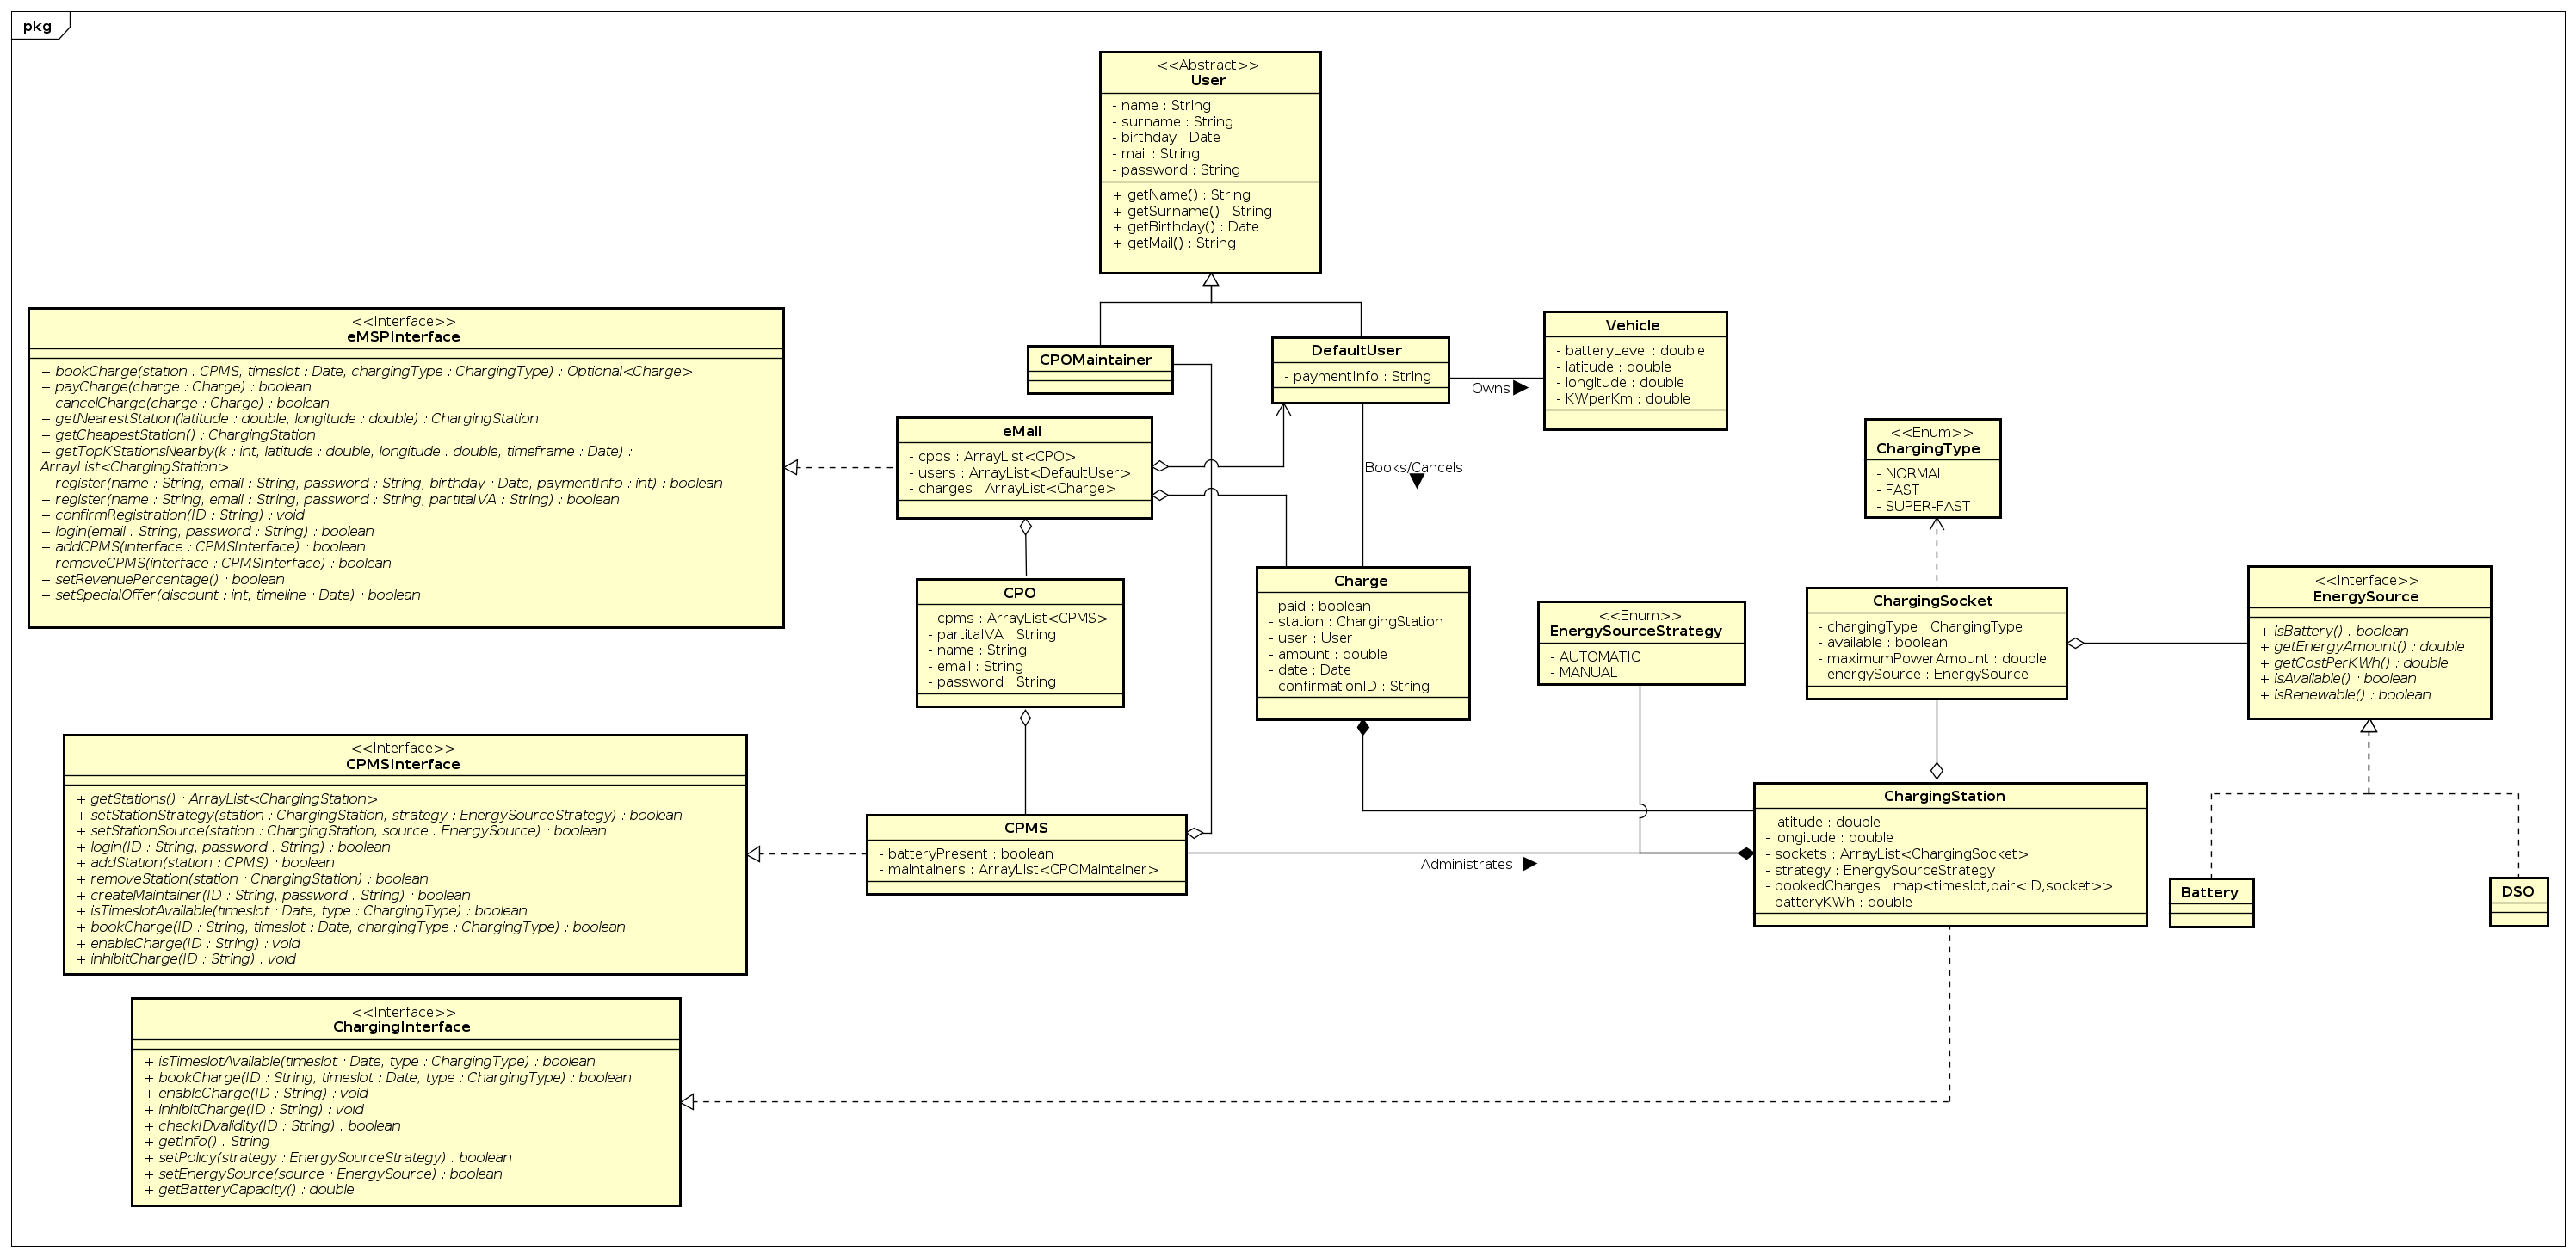
\includegraphics[keepaspectratio, width=16cm]{UML.png}
            \caption{UML}
      \end{center}
\end{figure}

\subsubsection{Scenarios}
It is assumed that in S4,S5,S6,S7 the user is already logged in the system (S2)
\begin{enumerate}[label=S\arabic*]
      \item User Signs up:\\
            Lucy, wanting to use the system, opens the app, she is prompted to login or register,
            she chooses to register herself and inserts her personal info (email, password, birthday, payment information, );
            an email is sent with a link to confirm the activation of the account, if the link is clicked within
            the first 15 minutes the account is activated and the sign up is successful,
            otherwise it is considered failed and the process must be repeated.
      \item User Logs in:\\
            Jay, after signing up, opens the app and he is prompted to insert his email and password,
            if the given information are correct the login is successful and he obtain access to his account
            and the service of the apps, otherwise the login is unsuccessful and it must be repeated.
      \item User searches for stations:\\
            Robert, once logged in, inserts the location and the time frame to search for charging stations.
            Once submitted a list of available charging station is displayed, the list is ordered by the distance of the station
            from the desired location. Via a menu Robert can choose to order the station either via distance, price or charging type(super-fast,fast,normal);
            or to display unavailable station and set the maximum distance from the chosen location.
            Robert chooses a station obtaining more detailed information.
      \item User books a charge:\\
            Jessica, after choosing a station, decides to book it, the station location and booked time frame are displayed
            and she is asked to confirm the booking via a popup. Jessica then receives a confirmation email with the details
            of the charge (Location, time frame, socket id) and a confirmation pin to insert at the station.
      \item User cancels a charge:\\
            Luke, after booking a charge wants to cancel it, he opens the app, select the booking he wants to cancel,
            and press the Cancel button, a popup appear asking confirmation, if it is pressed the booking is removed,
            the station returns available and a confirmation email is sent to the user; otherwise the booking is still valid.
      \item User charges the car:\\
            Mary, after booking a charge, arrives at the station, she parks her car at the designed socket
            and plugs her car in, Mary then inserts the confirmation pin in the socket to start the charge.
            The socket displays on a monitor the status and the finishing time of the charge.
            Once the charge is finished Mary receives a notification of finished charge,
            she gets her car and complete the charge.
      \item User gets charging suggestion based on his calendar:\\
            Josh is a very busy man, is also an avid google calendar user,
            setting up every event with correct time and location.
            The service accessing his calendar finds the closest available charging station to each car movement,
            it connects to the car while driving and stores the last charge level and once the battery is below fifty percent Josh gets notified
            about the possibility to charge his car in an available time-slot and near his movement.
            Josh liking the idea open the app and confirms the booking.
      \item Cpo subscribes to the system:\\
            Judy, the CEO of a famous CPO, wants to subscribe it to EMAll to improve sales and to access the CPMS feature.
            She opens a Website and select to sign up, she inserts the name, partita iva, a master password and the stations of the CPO.
            For each station she has to insert the number of charging port, the presence of batteries and, if there are any,
            wether to use the CPMS automatic source selector or to choose the preferred energy source.
      \item Cpo updates info about its system:\\
            The sysadmin of a CPO, Andy, after logging in with the master password has access to his CPO.
            Here he can change the number of stations, for each station he can update the number of socket and the energy source.
            He can also create and update maintainer account inserting the ID and password. For each maintainer he can choose which station the maintainer can maintain.
      \item Cpo employee logs in the service:\\
            Brett a CPO employee wants to access the service, he connects to the site and inserts the ID
            and password, if correct he logs in; otherwise the procedure fails and must be repeated.
      \item Maintainer maintains his assigned stations\\
            Lisa, a maintainer at a cpo logs in the service, here she can see the info of each station assigned to her.
            For each station she can: check the status(functioning or not), choose the energy source, update the number of available sockets.
            She can monitor the consumes, profitability and the usage of a specified station.
\end{enumerate}

\subsection{Product functions}
In the following subsections the functions of each subsystem are described.

\subsubsection{\ac{eMSP}}
\paragraph{Accessing the \ac{eMSP}}
In order to have a personalized experience the system needs accounts. So a registration and login process is present. When registering it's required to give the system Name, Surname, e-Mail, Password and a Payment Method. For the login, an authentication with e-Mail and password is required.

\paragraph{Performing a charge}
The principal feature of the system is the ability to help the people to plan a charge for their cars efficiently. For this, people can see the availability of charging stations and choose where and in which time slot to charge the vehicle.
Also, if a user changes his mind, there is the possibility to delete a previously booked charge with no charge.
When the user arrives in the booked socket of the charging station, he has to insert the pin that the application displays in order to let the charging process begin.
Always through the application, the user is able to pay for the service thanks to the previously inserted payment method.
The system also notifies the user when the charging process is completed.

\paragraph{Retrieving informations about charging stations}
Whenever a user selects a charging station, various informations are shown in order to help the user to make a decision on which station to choose. Informations reguard location, price, a parameter on how green the energy provided is, special offers and availability of sockets in the station.

\paragraph{Get suggestions about the recharge of the vehicle}
An additional feature the system offers reguards a proactive suggestion about the recharge of the vehicle. Thanks to the connection of the application with the car and with the electronic calendar, the system is able to suggest to the user where and when to charge the vehicle in order to satisfy certain parameters chosen by the user. These may involve minimizing the cost of the recharge, minimizing the environment impact of our recharge, minimizing the distance from the scheduled appointments.


\subsubsection{\ac{CPMS}}
\paragraph{Accessing the \ac{CPMS} as \ac{CPO}}


\paragraph{Manage the energy source for a charging station}
% \paragraph{Choose manually to use the batteries}
% \paragraph{Choose manually to use the \acp{DSO} energy}
% \paragraph{Choose to make the \ac{CPMS} choose the energy source automatically}



\paragraph{Providing charging station informations for utilizators}
\paragraph{Providing charging station informations for maintainers}
\paragraph{Acquire informations about \acp{DSO} price}



\subsection{User characteristics}

\subsection{Assumptions dependencies and constraints}
\subsubsection{Assumptions}
\begin{enumerate}[label=DA\arabic*]
      \item Users insert genuine data in the forms
      \item Users(Including CPOs) do not use the system with malicious intent
      \item All the electric vehicles can be charged by all the stations (no incompatibility)
      \item All the user have an active internet and GPS connection always available while using the service
\end{enumerate}
\subsubsection{Constraint}
\begin{enumerate}[label=C\arabic*]
      \item If a User wants to change the time slot of a charge he is required to cancel and re-book the charge
\end{enumerate}

\clearpage